% Set the author and title of the compiled pdf
\hypersetup{
	pdftitle = {\Title},
	pdfauthor = {\Author}
}

\section{Course intro}

A smartphone is a mobile phone running a mobile operating system, with advanced
capabilities with regard to computing power and connectivity. They are much more
advanced than traditional feature phones, and have lots of features, including
cameras, multimedia functionality, GPS, touch screens etc.

There are three main mobile operating systems in use today:

\begin{description}
  \item \textbf{Android}\\
  	Founded in 2003 by Andy Rubin and backed by Google. It's mostly free and
  	open source, and holds a very strong position in the market.
  \item \textbf{iOS}\\
  	Introduced in 2007 by Apple, this is a closed source operating system. The
  	first iOS phones were very groundbreaking in terms of their technology, and
  	were the first to feature touch screens, which are now ubiquitous in the
  	market.

\marginpar{Blackberry, Symbian, Palm OS etc could be listed here too.}

  \item \textbf{Windows Phone}\\
    Version seven was released in 2010, previous versions were terrible (imho).
\end{description}

\subsection{What's in a smartphone?}

Modern smartphones are jam packed with technology, containing cameras,
multimedia, GPS, high resolution touch screens, motion sensors, bluetooth, RFID,
NFC and even more stuff besides. They let you talk over multiple different
networks (2G, 3G, 4G etc), and access data using the same methods.

Of course, the millions of apps available for them is also a massive attraction.

Smartphones Operating Systems need to be very advanced in order to step up to
the tasks required of them by users. They need to be multitasking, to run lots
of different apps, and interface with the typical hardware a normal computer
might use (DMA, standard (ish) input devices etc). However, they also need to
have real-time elements in, since they must be able to drive sound, IO, radio
communications, digital signal processing etc

% Lecture two
\section{Signals in mobile systems}

Signals such as speech and music arrive at the device as physical, analogue
quantities that vary in a continuous manner over time. If we plot a graph of
voltage over time, then we get a waveform for that signal. We can convert
analogue signals to \textit{discrete time signals} by sampling them at set
intervals (discrete points in time). This produces a list of numbers from
$-\inf$ to $\inf$.

\subsection{Generating waves}

In order to create a wave with a period of $T$ seconds, you can use the formula:

\[
  y = sin(\frac{2\pi x}{T})
\]

Of course, since $f = \frac{1}{T}$, the frequency of the wave is the reciprocal
of the time period.

\subsection{Sampling waves}

We can work out the frequency of a wave, by finding how many complete cycles it
undergoes in one thousand samples, and multiplying that by the sample rate. For
example, if a wave has ten cycles from $1000$ samples at $30,000Hz$, then its
frequency will by $\frac{10}{1000} \times 30,000 = 300Hz$. This is visible in
Figure~\ref{discrete-signal}.

\begin{figure}
  \centering
  \begin{tikzpicture}
    \begin{axis}[%
      domain = 0:1000,
      samples = (\samplesScaleFactor * 1000),
      xlabel={Sample number},
      ylabel={Sample value (an integer)}]
      \addplot[black,thin] {sin(x * pi * (1080/1000))};
    \end{axis}
  \end{tikzpicture}
  \label{discrete-signal}
  \caption{1000 samples of an analogue sin wave of frequency $300Hz$ sampled at
  $30,000$Hz.}
\end{figure} 

Not all waves are so easy to analyse, rarely will a wave be at just one
frequency, instead, they are usually `noisy' and will be composed of many waves
added together. Many waves (that aren't just noise) will have a discernible
frequency that you can extract. The `extra' waves on top of this frequency
aren't necessarily bad, they might add harmonics, or texture to a sound.

\subsubsection{The Sampling Theorem}

\marginpar{Also known as \textit{Nyquist criterion}.}

The Sampling Theorem states that if a signal has all of its spectral energy
below $B$Hz, and is sampled at $F$Hz, where $F \geq 2B$, then it can be
reconstructed \textit{exactly} from the samples and nothing is lost.

In other words, if you are sampling a signal at \textit{less than half} of the
maximum frequency of the signal, then you won't be able to fully reconstruct the
signal from the samples, and you will get distortion.

Since music is usually sampled at $44.1$\si{\kilo\hertz}, we can accurately
sample music with frequencies up to around $22$\si{\kilo\hertz}. Speech rarely
has frequencies above $3.4$\si{\kilo\hertz}, so the sample rate for it can be
much lower, as we will see later on in the course.

\subsubsection{Aliasing}

If we sample at less than twice the frequency of the wave, then we will get
distortion, known as aliasing. The first lab on this course relates to aliasing.
Even if we don't want frequencies higher than half our sample rate, we need to
filter them out anyway, since otherwise, we will get aliasing when we sample
them.

To be precise, if a wave of frequency $f$ is sampled at a frequency of below
$2f$ (lets call this $F$, then the sampled output will be a wave of frequency $F
- f$.

For example, if we sample a $6\si{\kilo\hertz}$ wave at a frequency of $10\si{\kilo\hertz}$, when we will
get a wave of frequency $10-6 = 4\si{\kilo\hertz}$.

This is bad, because if you have harmonics in a musical note that are higher
than half the sampling frequency, then these harmonics will be out of tune post
sampling, and will go down when it's supposed to go up.

It may be hard to work out exactly why aliasing occurs, but
Figure~\ref{aliasing}, showing a $6\si{\kilo\hertz}$ wave sampled at $8\si{\kilo\hertz}$ makes it easier
to see:

\begin{figure}[H]
  \centering
  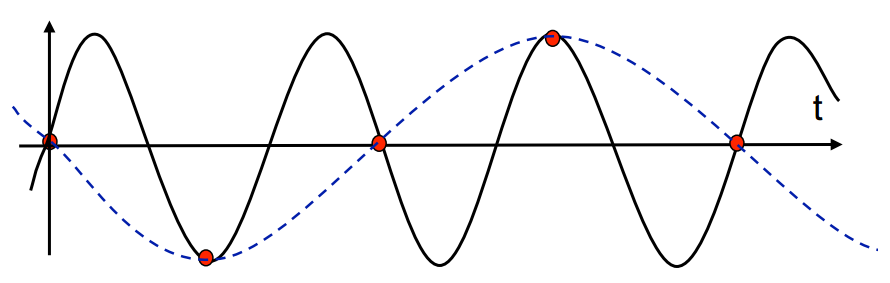
\includegraphics[width=\textwidth]{images/aliasing}
  \caption{A $6\si{\kilo\hertz}$ wave sampled at $8\si{\kilo\hertz}$ has a post-sampling frequency of 
  $2\si{\kilo\hertz}$}
  \label{aliasing}
\end{figure}

\subsection{Decibels}
\label{decibels}

Sound can be measured in decibels, which is a logarithmic ratio. The formula is
as follows:

\[
  \si{\decibel} = 10 \times log_{10}\left(\frac{s_1}{s_2}\right)
\]

If $s_1$ is twice as loud as $s_2$, then it will be $10\times\log_{10}(2)=3\si{\decibel}$
louder than $s_2$.

The following table shows the power ratio ($\frac{s_1}{s_2}$) against the
equivalent decibels:

\begin{center}
  \begin{tabular}{|l|l|}
    \hline
    \textbf{Power ratio} & \textbf{Decibels} \\ \hline
    $\frac{1}{2}$ & -3 \\ \hline
    $1$ & $0$ \\ \hline
    $2$ & $3$ \\ \hline
    $4$ & $6$ \\ \hline
    $10$ & $10$ \\ \hline
    $100$ & $20$ \\ \hline
    $1000$ & $30$ \\ \hline
    $10^{5}$ & $50$ \\ \hline
    $10^{10}$ & $100$ \\ \hline
  \end{tabular}
\end{center}

\section{Encoding and storing signals}

There are a variety of different ways to encode sound. The two main types of
coders for talking over the phone are \textit{waveform} coders, and
\textit{parametric coders} (sometimes called vocoders).

\begin{description}
  \item \textbf{Waveform coders}\\
  Waveform coders `operate on' the sound waves directly, and aim to change the
  wave so that it is transmitted in an optimal way. They are simple to
  understand and implement, but can't achieve \textit{really} low bit rates.
  They aim to preserve the exact shape of the wave.

  \item \textbf{Parametric coders}\\
  Parametric coders try and model human speech by exploiting how we produce
  sound with our vocal chords and mouth shape. They don't try and preserve the
  exact wave shape, but instead try and describe \textit{perceptually
  significant features} as sets of parameters. This is more complicated and
  harder to implement, but achieves lower bit rates.
\end{description}

Techniques that fall into both types of coder will be discussed in this section.

\marginpar{\textbf{Dynamic range} is the ratio between the loudest sound we can
hear, and the most quiet sound we can hear.}

Humans can hear frequencies between $20\si{\hertz}$ and $20\si{\kilo\hertz}$,
and have a dynamic range of $120\si{\decibel}$. We can represent six decibels
per bit of information using uniform quantisation (see section~\ref{uniform-quantisation}),
so we need about $\frac{120}{6}$ bits to properly represent the sample.

\subsection{Bitrates in different settings}

Sometimes, 20 bits per sample is too much, so different bit rates are used in
different applications:

\begin{description}

  \item \textbf{CD's}\\
  Unfortunately, 20 bits per sample was too much for CD's (you wouldn't be able
  to fit enough songs on each CD), so instead, 16 bits item per sample was
  adopted as the standard. In order to `lose' these four bits, we make the quiet
  bits of the songs louder (since we probably wouldn't be able to hear them
  anyway).

  As a consequence of this, a song on a CD plays at a rate of $16 \times 44100
  \times 2 = 1411\si{\kilo\bit\per\second}$.

  \item \textbf{Landlines}\\
  \marginpar{In practice, sometimes, vowel sounds like `f' and `s' can be mixed
  up.}
  Landlines are band-limited to a range of frequencies from $50\si{\hertz}$ to
  $3.4\si{\kilo\hertz}$. Obviously, this is much, much less than the dynamic
  range that humans can hear, but we only usually talk in frequencies covered by
  the range provided. This means that the sound will lose its `naturalness' but
  not intelligibility (supposedly).

  \marginpar{\textbf{Band limiting} is when a sound is Fourier transformed, and
  frequencies above or below a certain frequency are stripped.}

  The sample rate for telephone quality speech is $8\si{\kilo\hertz}$, with
  $8\si{\bit\per}s$. This gives a bitrate of $64\si{\kilo\bit\per\second}$. In
  order to use just $8\si{\bit}$ per sample, we need to use non-uniform
  quantisation (like in the (second?) lab), such as $\mu$-law quantisation.

  \item \textbf{Mobile Telephones}\\
  Mobile phones use a bit rate that changes based on factors such as the signal
  quality, but has a minimum value of $4.75\si{\kilo\bit\per\second}$, and a
  maximum value of $12.2\si{\kilo\bit\per\second}$. AMR encoding (see
  Section~\ref{amr}) is used to achieve such low bitrates.

\end{description}

\subsection{Quantisation}

When we've sampled a wave, if we leave all of our readings as floating point
numbers, then we could be using a lot of space to store each sample. We could
slightly reduce the quality of our sound by \textit{quantising} it. This is when
you map the continuous values onto a range of integers, where the range of
integers spans a power of two (so you can use as few bits as possible).

You can see that the third wave in Figure~\ref{quantised-wave} has been
quantised into five integers, since there are five discrete values in the
waveform ($0,1,2,3,4$) (requiring four bits), and there will be an extra bit to
indicate the sign. If whoever made the diagram was trying to be as efficient as
possible, they might have had either one less value (so that the numbers could
be represented in three bits), or made full use of the four bits for the value,
and used values from $0-7$.

\begin{figure}[H]
  \centering
  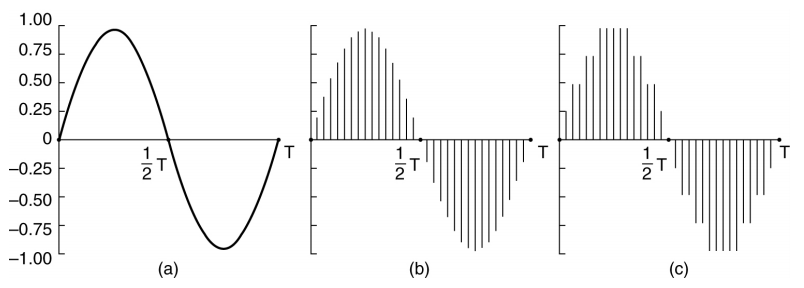
\includegraphics[width=\textwidth]{images/quantised-wave}
  \caption{An analogue wave (a), after its sampled (b), and once it's been quantised (c)}
  \label{quantised-wave}
\end{figure}

Quantisation produces noise (known as quantisation noise), since errors are
introduced in the process. If there are many bits per sample (e.g. 16), then
this error will be small, but if you only used say, five bits, then the error
would be noticeable. As a consequence of this, we have to work a trade-off
between storage capacity or bandwidth and quality.

There are two types of quantisation, uniform and non-uniform:

\begin{description}
  \item \textbf{Uniform quantisation}\\
  \label{uniform-quantisation}
  A simple type of quantisation, each binary number represents a voltage, where 
  incrementing the binary representation will correspond to an increase in the 
  voltage of $\Delta\si{\volt}$, called the \textit{quantisation step-size}.

  It might be hard to decide on a value for $\Delta$, because different sounds
  will span different ranges of amplitude as shown in Figure~\ref{choosing-delta}.

  \begin{figure}
    \centering
    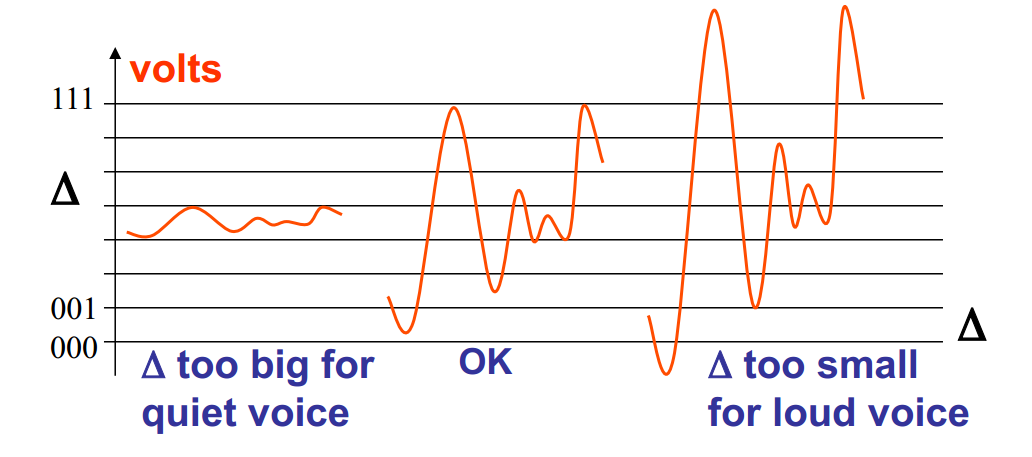
\includegraphics[width=0.8\textwidth]{images/choosing-delta}
    \caption{This waveform shows how a a bad choice for $\Delta$ can adversely
    affect the quality of the sound, when it is undergoing uniform quantisation.}
    \label{choosing-delta}
  \end{figure}

  One solution to this, is to adjust the value of $\Delta$ on a sample-to-sample
  basis. This uses up extra bandwidth though, so is not a preferred solution.

  \item \textbf{Non-uniform quantisation}\\
  \label{non-uniform-quantisation}
  Non-uniform quantisation is when the quantisation step-size is not the same
  between different quantised values, as evidenced in
  Figure~\ref{fig-non-uniform-quantisation}.

  \begin{figure}
    \centering
    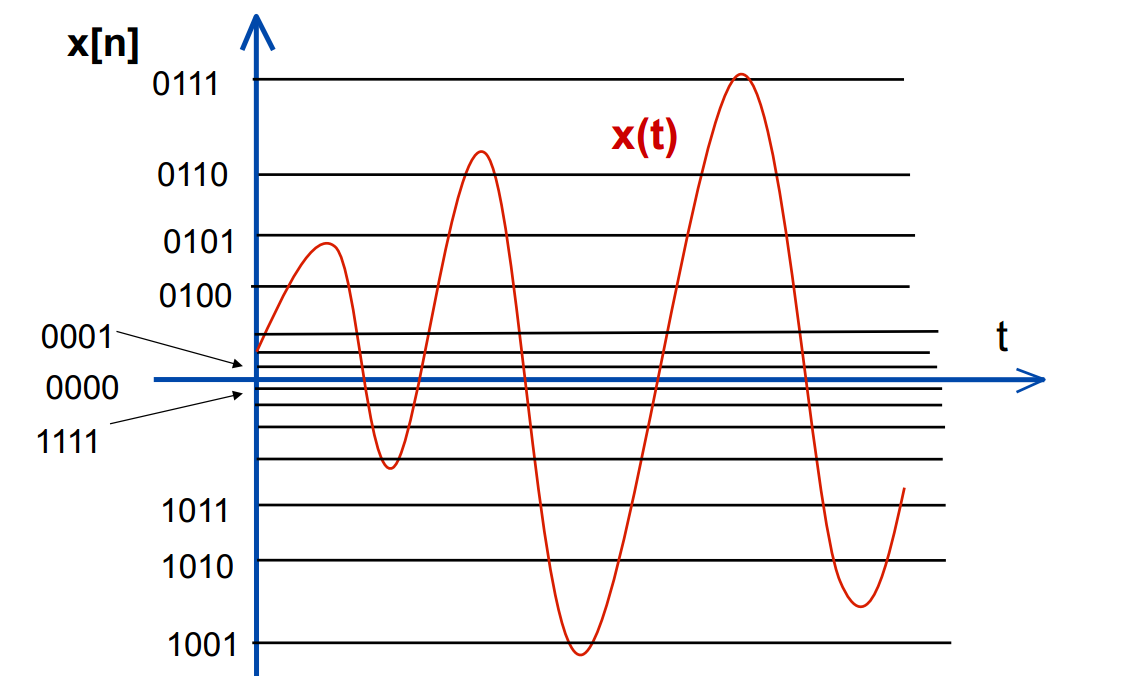
\includegraphics[width=0.5\textwidth]{images/non-uniform-quantisation}
    \caption{An example of non-uniform quantisation.}
    \label{fig-non-uniform-quantisation}
  \end{figure}

  Non-uniform quantisation is implemented like so:

  \begin{enumerate}
    \item Apply accurate uniform quantisation.
    \item Apply a `compranding' formula, such as $\mu$-law.
    \item Uniformly quantise again using fewer bits.
    \item Transmit.
    \item Reverse the process of steps three and two with an `expander'.
  \end{enumerate}

  \marginpar{Compranding is just a coding technique similar to compression. It
  doesn't increase the quality of the sound or anything (though it might do if
  the alternative was to use the same number of bits with uniform quantisation.)}

  A `comprander' will increase the value of small samples, and decrease the
  value of large samples, and an `expander' just does the reverse. Even though
  we only apply two uniform quantisations, the comprander and expander mean the
  overall effect is one of non-uniform quantisation.

  % TODO: Mu law and A-law

\end{description}

\subsubsection{Quantisation error}

Quantisation Error is produced when we quantise a wave, and is random in the
range of $\pm\frac{\Delta}{2}$. Since the error is random, the error is heard as
white noise, and is spread evenly across all frequencies. The Mean Square Value
(MSV) of the noise, is $\frac{\Delta^2}{12}$.

We can calculate the Signal to Quantisation Noise Ratio (SQNR), which is how
loud the signal is in comparison to the noise (hence it is given in decibels -
see Section~\ref{decibels}). To do this, we use the formula:

\[
  \text{SQNR} = 10\log_{10}\left(\frac{\text{MSV of signal power}}{\text{MSV of noise}}\right)
\]

We can use this formula to calculate the $\si{\decibel\per\bit}$ for sending
telephone data (speech, text etc):

\begin{mymulticols}
\[
  \text{SQNR} = 10\log_{10}\left(\frac{A^2 / 2}{\Delta^2 / 12}\right)
\]

The maximum amplitude of a sine wave that has been quantised with a step size
of $\Delta$ is $\frac{2^{bits}}{2}\Delta$

\allowdisplaybreaks
\begin{align*}
  &= 10\log_{10}\left(\frac{\left(\frac{2^{bits}}{2}\Delta\right)^2 / 2}{\Delta^2 / 12}\right)\\
  &= 10\log_{10}\left(\frac{\left(2^{2 \times bits - 2}\Delta^2\right) / 2}{\Delta^2 / 12}\right)\\
\end{align*}
\begin{align*}
  &= 10\log_{10}\left(\frac{\left(\frac{2^{2 \times bits}}{4}\Delta^2\right) / 2}{\Delta^2 / 12}\right)\\
  &= 10\log_{10}\left(\frac{\frac{2^{2 \times bits}}{8}\Delta^2}{\Delta^2 / 12}\right)\\
  &= 10\log_{10}\left(\frac{\frac{2^{2 \times bits}}{8}}{1 / 12}\right)\\
  &= 10\log_{10}(1.5 \times 2^{2 \times bits})\\
  &= 10\log_{10}(1.5) + 10\log_{10}(2^{2 \times bits})\\
  &\approx 1.8 + 10\log_{10}(2^{2 \times bits})\\
  &\approx 1.8 + (6 \times bits)\\
\end{align*}
\end{mymulticols}

This only strictly applies for uniformly quantised sine waves, but also holds
fairly well for speech and music.

If an 8 bit uniform quantisation scheme is designed for loud talkers (so they
will use all eight bits), then it will have a SQNR of $(6\times 8) + 1.8 =
49.8$. If another talker is much quieter, and talks $30\si{\decibel}$ quieter,
then the samples will be encoded using only $3$ bits:

\begin{align*}
  6 \times bits - 1.8 &= 49.8 - 30\\
  6 \times bits &= 48 - 30\\
  6 \times bits &= 18\\
  bits &= 3
\end{align*}

\marginpar{Remember, since the SQNR is calculated by
$\frac{\text{MSV of signal power}}{\text{MSV of noise}}$ it has an inversely
proportional relationship with the amount of noise. I.e. will go up as the noise
decreases.}

Since the quantisation noise for three bits is much lower ($19.8\si{\decibel}$)
for the quietly talking person, they will probably be able to hear the noise
over the phone.

For the loudest CD quality (16 bit) music, the maximum SQNR value is
$97.8\si{\decibel}$, whereas for the most quiet sounds, it is
$-22.8\si{\decibel}$ (which means the noise is louder than the actual sound).
Obviously this isn't ideal, so we need to apply DRC (Dynamic Range Compression)
improve the balance.

\subsection{Differential encoding}

A sample of audio isn't just random data, and since the data represents a wave,
consecutive values are likely to be relatively close together. If that is the
case, then maybe we could encode the data as the difference between one sample
and the next. If the differences are easier to transmit than the raw data, then
we could save resources such as bandwidth. Such an encoder is shown in
Figure~\ref{differential-encoder}.

\begin{figure}
  \centering
  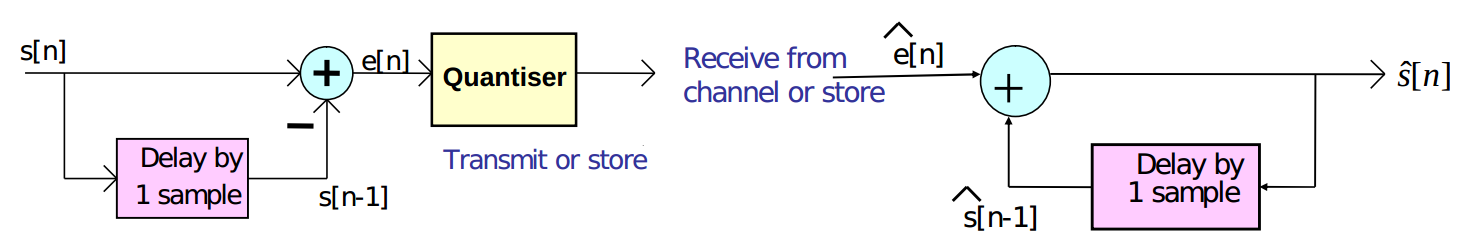
\includegraphics[width=\textwidth]{images/differential-encoder}
  \caption{An example of how a differential encoder might both encode and decode
  audio samples.}
  \label{differential-encoder}
\end{figure}

\marginpar{PCM stands for Pulse Code Modulation, and is basically the same as
what we mean by quantisation.}

This is known as Adaptive Differential PCM, and can be made to work at bitrates
of $16-32\si{\kilo\bit\per\second}$. However, for use in mobile telephones, we
need a bit rate that is at least four times lower than this\dots

\subsection{Linear Predictive Speech Coding}

\marginpar{Voiced speech is normal speech, unvoiced speech is whispering. If
normal speech is sampled, then some of it will be classed as unvoiced, since
only vowel sounds actually require the use of vocal chords (try it!).}

LPC is a type of parametric encoder. Working on the principle that voiced speech
is created by the vocal chords opening and closing at frequencies that change
over time, the coder can send the fundamental frequency of the noise as well as
parameters (called coefficients here) modelling the shape of the mouth over the
network to recreate the speech at the receiver.

The sender derives the parameters at a rate of $50\si{hertz}$, which include how
loud the speech is, the coefficients modelling the vocal tract, and the
fundamental frequency of the sound. Figure~\ref{LPC} shows how these parameters
are used to reconstruct the speech at the receiver.

\begin{figure}
  \centering
  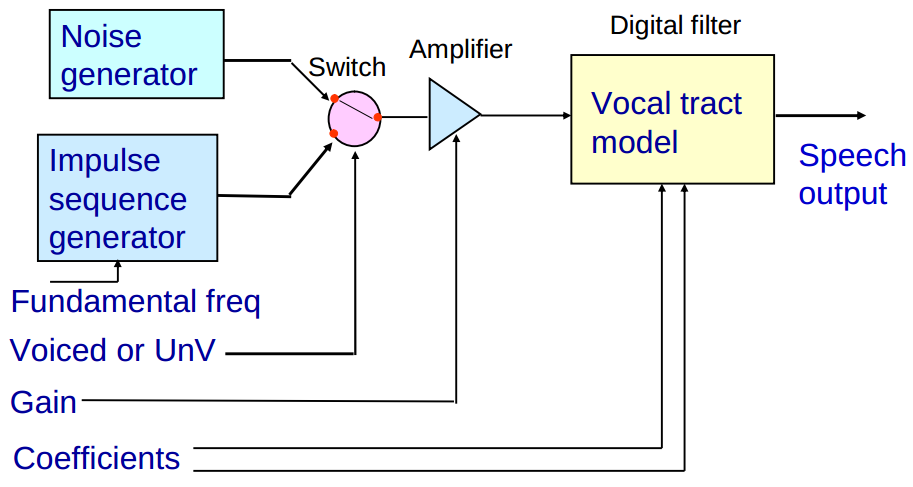
\includegraphics[width=\textwidth]{images/LPC}
  \caption{An implementation of a Linear Predictive Speech Decoder}
  \label{LPC}
\end{figure}

\subsubsection{LPC-10}

LPC-10 was a coder once used by the military that had a bit rate of
$2.4\si{\kilo\bit\per\second}$. Each $20\si{\milli\second}$ frame has the
following components:

\begin{tabular}{l l}
  37 bits & Ten filter coefficients\\
  1 bit & Voiced/unvoiced decision\\
  8 bits & Gain (the amplitude)\\
  8 bits & Fundamental frequency\\
\end{tabular}

\marginpar{MIPS is Millions of Instructions Per Second}

This made for a total of $56\si{\bit}$ per frame. Although it's easy to
understand and implement, and requires little processing power (according to
Wikipedia\footnote{\url{http://en.wikipedia.org/wiki/FS-1015}}, it requires
$20$MIPS and $2\si{\kilo\byte}$ of RAM).

\subsubsection{Codebook Excited LPC}

Codebook Excited LPC (CELP) is a way of further reducing the bandwidth used by
LPC. The principle is that there are a number of pre-configured parameters that
the receiver and sender have stored in a `codebook', and the sender just sends
the index of the one that is most similar to the sound that it is trying to
produce.

It finds the most similar sample using `analysis by synthesis', which involves
trying all the entries in the codebook one by one, and sending whichever is the
closest to the one we want. 

CELP is used in commercial mobile telephones, and is utilised by the
\textbf{Adaptive MultiRate} (AMR) coder for rates at
$12\si{\kilo\bit\per\second}$ or lower.

\subsection{Comfort noise}

When a two way conversation is going on, and neither party are speaking, nothing
will be played through the speakers to either party (since we don't transmit
quiet sounds since that wastes power). To mitigate this, the phones will
generate and insert `comfort noise' which is psudorandom background noise that
sounds like whatever is going on at the other end of the phoneline. Each phone
will determine if its owner is silent, and transmit the characteristics of the
background noise using very few bits if they are so that the other phone can
recreate a similar background noise for the other person.

\subsection{Error correction, detection \& prevention}

Mobile systems are affected by errors in the transmission of data, often in the
form of noise affecting radio reception. There are many ways of
avoiding/mitigating errors, the most important ones looked at in this course
are; Forward Error Correction (FEC) and error detection and retransmission
(Automatic ReQuest).

\subsubsection{Forward Error Correction}

We can build redundancy into the transmission by appending check bits or some
other form of coding that will bloat the size of the transmission, but result in
less errors.

We can use block coding or convolutional coding to implement this. \textbf{Block
coding} is when you process the data in blocks (well duh), which requires you to
encode the whole block at the transmitter and decode it again at the receiver.
You can't use a block unless it's been fully decoded. \textbf{Convolutional
coding} on the other hand can yield usable bits soon as just a few of the
transmitted bits arrive at the receiver. Convolutional coders treat data as a
stream, whereas block coders deal with data in chunks.

Here are some examples of the above:

\begin{description}
  \item \textbf{Repeating bits}:\\
    We could simply send bits a few times, instead of just once and take the 
    mode of them at the receiver. If we sent three bits for every bit, then
    if there was one bit error, then it would be fine since we could take the 
    majority of the received bits, and the one error bit would be ignored.

    The number of repeats must be an odd number, otherwise we could end up with 
    a half and half split.
  \item \textbf{Parity}\\
    As a simple (and not very effective) way of detecting bit errors, we could
    append a parity bit to the end of blocks. The parity bit would be \texttt{0}
    if the block had an even number of ones, and \texttt{1} if it had an odd
    number of ones. If we have an $n$ bit number, we can calculate the parity
    using $n - 1$ \texttt{XOR} operations; $b_0 \oplus b_1 \oplus \dots \oplus
    b_n$.

    When the receiver gets the bits, the parity of all of them (including the
    parity bit) must be computed. If the parity is \texttt{1}, then some bit
    error definitely occurred, whereas if it is \texttt{0}, then the data
    \textit{may be} correct (but there could be two or more errors as well).

    Parity checking is a block code, since you need to wait for the whole block
    to arrive before checking the parity.
  \item \textbf{Hamming distance}\\
    The Hamming distance between two binary numbers is the number of bits that
    are different. This is obtained by \texttt{XOR}ing the two numbers together
    and counting the number of ones. This is useful if we want to know how many
    bit errors it takes to convert one number to another.

    You have a set list of code words that you can use, each with a minimum
    hamming distance from it to any other. Then, you can detect and even errors
    by comparing your received code to the allowed ones.

    Figure~\ref{HammingCodes} shows an implementation.

    \begin{figure}
      \lstinputlisting[style=java]{examples/hamming_code/HammingCode.java}
      \label{HammingCodes}
      \caption{A Java implementation of HammingCodes}
    \end{figure}

    Hamming codes are block codes, since you need the whole block to calculate
    the distance between the received block and the ones in the codebook. It is
    common practice to introduce check bits onto code words to make the distance
    larger.

    The notation for Hamming Codes is $(m+r, m)$, where $m$ is the number of
    message bits, and $r$ is the number of check bits. The $r$ bits are appended
    to the end of the code words, and are derived from the value of the $m$
    bits. For example, with a $(7,4)$ hamming code, we could make:

    \begin{itemize}
      \item $r_0$ = $m_0 \oplus m_1 \oplus m_2$
      \item $r_1$ = $m_0 \oplus m_1 \oplus m_3$
      \item $r_2$ = $m_0 \oplus m_2 \oplus m_3$
    \end{itemize}

    This would give a \textit{syndrome table} (i.e. correction table) of:

    \begin{center}
      \begin{tabular}{|>{$}l<{$}|>{$}l<{$}|>{$}l<{$}|l|}
        \hline
          r_0 & r_1 & r_2 & Correction to\\ \hline
          0   & 0   & 0   & None\\ \hline
          0   & 0   & 1   & $r_2$\\ \hline
          0   & 1   & 0   & $r_1$\\ \hline
          0   & 1   & 1   & $m_1$\\ \hline
          1   & 0   & 0   & $r_0$\\ \hline
          1   & 0   & 1   & $m_2$\\ \hline
          1   & 1   & 0   & $m_3$\\ \hline
          1   & 1   & 1   & $m_0$\\ \hline
      \end{tabular}
    \end{center}

  \item \textbf{Interleaving}:\\
    Since bit errors in radio links often occur in bursts (e.g. caused by a car
    turning on), we could transform one dimensional blocks of data into two
    dimensional matrices, and transfer them column by column. This way, if there
    is a `bursty' bit error, then it will affect multiple rows, but the bit
    error correction (such as) the repeating method, or hamming codes could
    detect the error since only one or two bits may be wrong, not all of them.
\end{description}

\subsubsection{CRC checks}

A Cyclic Redundancy Check is a block code for detecting bit errors. If we find
the value of the number we're transmitting in decimal and divide it by a number
such as seven, we can append the remainder onto the message. Then at the
receiver, we can divide the received bits again and if we get a different
remainder, then we know that a bit error has occurred.

If the bit errors happened to add or subtract the number that you were dividing
by, then the remainder would be the same and you would not be able to detect the
errors. If we make the number large, then this is unlikely.

Real CRC checks use \textit{Galois Field Arithmetic}\footnote{
\url{http://en.wikipedia.org/wiki/Finite_field_arithmetic}} to do the maths,
since binary numbers can be expressed as polynomials:

\begin{description}
  \item \textbf{Summing}:\\
    To calculate the sum of two binary numbers, we can just XOR their bits.
    Subtracting is the same:
N
    \[
      1001 \oplus 0111 = 1110
    \]
  \item \textbf{Long division}:\\
    %TODO: Understand this
\end{description}

There are three CRC generators used in practice:

\begin{itemize}
  \item CRC-8-ATM: $x^8 + x^2 + x + 1$
  \item CRC-16-IBM: $x^{16} + x^{15} + x^2 + 1$
  \item CRC-32-IEEE: \textbf{Quite long...}
\end{itemize}

A generator of order $r$ can detect all error bursts of length $\leq r$.

\subsubsection{Convolutional Coders}

If we are processing streams of data, then we could have a `rolling parity
check'. When we encode, the previous $n$ bits are \texttt{XOR}'d together to
produce another stream of bits. We can then interleave the new parity stream
with the normal stream.

At the decoder, the bits are valid if each of the parity bits (i.e. not the
normal ones) is the \texttt{XOR} of the previous three normal bits. If the bit
sequence is invalid, then we can select the valid sequence with the minimum
Hamming distance to the received sequence and therefore have error correction.

With sequences of around 8 bits, that is fine, since there would be 256 valid
sequences of 16 bits long each, however, for longer sequences (e.g. 1024 bits),
then this would not be feasible.

\marginpar{Convolutional coders that encode bit streams are called
\textit{rolling parity} coders.}

A soft decision decoder is where if we're unsure as to what the value of a bit
is, then we could use previously known probabilities to determine what we could
pick.

%TODO: Understand convolutional coders a bit better...

\subsubsection{Miscellaneous FEC stuff}

Well thought out use of FEC techniques in mobile systems increases the energy
efficiency and effectiveness of the system. Transmitting at higher power is one
way of reducing errors in the system, but `loud' signals also cause lots of
interference over a wider range and, of course, uses lots of battery. FEC lets
us reduce the transmission power, yet overcome the bit errors that come as a
result, which allows us to re-use different frequencies and reduce power
consumption.

We could increase the bit rate by not encoding in binary, but using any $2^n$
number of states. If we could send the values $\{0,1,2,3\}$, then we could send
two bits per pulse, effectively doubling our bandwidth. This is limited by the
noise in the channel.

The \textbf{Shannon-Hartley Law} says that the channel capacity $C$ is equal to:

\[
  C = B \log_2(1 + \frac{S}{N}) \si{\bit\per\second}
\]

Where $B$ is the bandwidth in $\si{\hertz}$, and $\frac{S}{N}$ is the signal to
noise power ratio.

% Lecture 6

\section{Mobile networks}

Since their inception, the desired use of cellular networks has changed from
being solely about transmitting speech, to transmitting textual data, and now
arbitrary packets. This has required them to evolve from `circuit switched
networks', where (at a fundamental level) a physical connection must be made
between wires to facilitate data transfer, to `packed switched networks'.

This evolution is really interesting, since circuit switching originated from
landline phones, but packet switching was from digital networking such as
Ethernet. As the technology has progressed, cellular data has moved towards the
Internet's way of doing things.

However, mobile phones have moved on from being single feature devices, merely
letting you call other users. Now they are \textit{smart}phones, and this
requires them to use a plethora of different technologies to be able to fulfil
user's demand; GPS, bluetooth, radio etc to name a few.

\subsection{Cellular networks}

One reason why mobile phones can work so well is that they take advantage of
\textit{spatial multiplexing}. This divides an area into small areas called
cells, each having a frequency band. The cells are different sizes based on
their expected usage rates (cells will be more dense in areas with more
demand). Frequency bands are re-used when a cell with the same frequency band is
far enough away, and because of this, mobile phones must take care not to
transmit their signals too loud and pollute the spectrum for nearby cells.

\marginpar{Cells are typically $0.1-35\si{\kilo\meter}$ in diameter. Obviously
small cells are better since they will handle more users per unit area (assuming
cell size is independent of user capacity), but users will need to transmit at a
lower power (so the neighbouring cells using the same frequency aren't
affected). This is actually a good thing sometimes, since it uses less battery,
and we can use FEC to mask bit errors.}

Breaking the spectrum up into frequencies, and mapping that onto physical cells
is a nice concept - and it works very very well in reality, but it does have
some drawbacks; for example, what happens when a user moves into a different
cell while on the phone? Thankfully, the system supports transparent and
seamless handovers as the user moves from cell to cell.

\subsubsection{The evolution of cellular}

Cellular networks have gone through four iterations to date, with a fifth one
coming in the future:

\begin{description}
  \item %TODO: Slide 6 from lecture 6
\end{description}

\section{Frequency Domain Processing}

Instead of processing waves, and parts of waves, how about we turn them into
frequencies and process those instead? Frequencies are a lot easier to deal with
in many ways since they are easier to understand and smaller to store.

\subsubsection{Sinusoids}

A sinusoid is a sine wave delayed by $D$ seconds, and is given by the formula:

\[
  y = M \times cos(2\pi F (t - D))
\]

Figure~\ref{fig-sinusoid} shows two sinusoids; one where $D = 30^{\circ}$ and
another where $D = 0$.

\begin{figure}
  \centering
  \begin{tikzpicture}
    \begin{axis}[%
      width=\textwidth,
      xtick={
        -360, -270, -180, -90, 0,
        90, 180, 270, 360
      },
      ytick={-1,0,1},
      yscale=0.4,
      domain = -360:360,
      samples = (\samplesScaleFactor * 1000),
      xlabel={},
      ylabel={}]
      \addplot[black,thin] {cos(2 * (x - 30)};
      \addplot[red,thin, dashed] {cos(2 * (x - 0)};
    \end{axis}
  \end{tikzpicture}
  \label{fig-sinusoid}
  \caption{1000 samples of a sinusoid where $D = 30^{\circ}$ (black) and where
  $D = 0$ (dotted red).}
\end{figure} 

Figure~\ref{fig-sinusoid} is a simple sine wave, but any wave (such as the one
in Figure~\ref{fig-complex-wave}) that is periodic can be found to have a
fundamental frequency of $\frac{1}{T}$, where $T$ is the period of the wave. A
recording of a voice, or musical instrument may be found to have a similar
waveform to that of Figure~\ref{fig-complex-wave} as long as we `zoom in' to a
segment short enough that any gradual change in frequency is negligible. This is
called \textbf{psudo-periodicity}.

\begin{figure}
  \centering
  \begin{tikzpicture}
    \begin{axis}[%
      width=\textwidth,
      xtick={
        -360, -270, -180, -90, 0,
        90, 180, 270, 360
      },
      ytick={-1,0,1},
      yscale=0.4,
      domain = -360:360,
      samples = (\samplesScaleFactor * 1000),
      xlabel={},
      ylabel={}]
      \addplot[black,thin] {(1.0 * cos(2 * (x - 30) * 1)
                          + (0.2 * cos(2 * (x - 00) * 4)
                          + (0.2 * cos(2 * (x - 60) * 1.3))};
    \end{axis}
  \end{tikzpicture}
  \label{fig-complex-wave}
  \caption{A complex wave with a frequency of
  $\frac{1}{180} = 0.00\overline{5}\si{\hertz}$}
\end{figure} 

\subsubsection{Fourier Series}

Any periodic wave of frequency $F$ can be written as:

\begin{align*}
  x(t) = A_0 / 2 &+ A_1 cos(2 \pi Ft) + B_1 sin(2\pi Ft)\\
                 &+ A_2 cos(2 \pi 2Ft) + B_2 sin(2\pi 2Ft)\\
                 &+ A_3 cos(2 \pi 3Ft) + B_3 sin(2\pi 3Ft)\\
                 &+ \dots
\end{align*}

This is sometimes called its `cos and sin' form, but we could re-write it as:

\[
  x(t) = \frac{M_0}{2} + \sum\limits^\infty_{k=1}M_k\cos(2\pi (kF)t + \phi_k)
\]

Here, each time the summation iterates, we are adding the next harmonic of the
sound. The fundamental frequency $F$ is the first harmonic when $k=1$.

Because the harmonics get higher and higher, we can't sample the whole series
because otherwise the frequency of the harmonics will start to become higher
than half the sampling frequency and we will get aliasing (see
Section~\ref{aliasing}). In that case, we only go up to $k=\frac{N}{2} - 1$,
where $F(\frac{N}{2} - 1) \le \frac{Fs}{2}$. If we took $Fs$ samples every
second, then the formula would be:

\[
  x(n) = \frac{M_0}{2} + \sum\limits^{\frac{N}{2}-1}_{k=1}M_k\cos\left(2\pi (kF)\frac{n}{Fs} + \phi_k\right)
\]
\[
  \text{Where } n = 0,1,\dots,\text{size}(x)
\]

The more harmonics we compute, the closer we can get to reconstructing the wave
from them afterwards.

\subsubsection{Discrete Fourier Transform (iDFT)}

The DFT converts samples of length $n$ into $n/2 - 1$ samples and a `dc term'.
They are arranged in a length $n$ array, but the second half is the same as the
first half but reversed. The $0^{th}$ element of the array is the DC term, but
the $i^{th}$ element is the $i^{th}$ harmonic. 

The algorithm to convert from the time domain into the frequency domain is
\textit{N-point DFT}. To do the opposite, we can use the \textit{N-point inverse
DFT} algorithm.

DFT is used to:

\begin{itemize}
  \item Perform spectral analysis on a signal to find out what components are 
    present.
  \item Convert into the frequency domain before applying signal processing (and
    converting back again afterwards). For example, you could filter out noise 
    from a sine wave, since you could remove all frequencies with an amplitude
    below a certain level.
\end{itemize}

\subsection{Wav files}

Signals are stored in many different ways. One `easy' format, is the
\texttt{.wav} format. It is just a list of binary numbers, each representing a
single value of the wave at a discrete time.

% TODO: More formats, encoding etc
